\documentclass[a4paper, 14pt]{extreport}
%--------------------------------%
% فایل حاوی فراخوانی بسته‌ها و تعریف دستورات و تنظیمات لازم 
% بسته‌های مورد نیاز
\usepackage{graphicx}
\usepackage{titlesec}
\usepackage{tocloft}
\usepackage{amsmath}
\usepackage{amsthm}
\usepackage{amssymb}
\usepackage{amsfonts}
\usepackage{float}
\usepackage{array}
\usepackage{multirow}
\usepackage{subcaption}
\usepackage[T1]{fontenc}
\usepackage[chapter]{algorithm}
\usepackage{tcolorbox}
\usepackage{xcolor}
\usepackage{xhfill}
\usepackage{listings}
\usepackage{DejaVuSansMono}
\usepackage{enumitem}
\usepackage{comment}
\usepackage{fancyhdr}
\usepackage{tabularx}
\usepackage{tablefootnote}
%بسته‌ی پیوست و تنظیمات لازم آن
\usepackage[toc]{appendix}
\renewcommand{\appendixname}{پیوست}
\renewcommand{\appendixtocname}{پیوست‌ها}
%بسته‌ی لازم برای تنظیم حاشیه‌های صفحات
\usepackage{geometry}
% setting the the margins of the paper 
% inner and outer are different for right to left writings 
% en inner 2/5  + 0/5 gutter cm ~ fa outer 2/5 cm 
% en outer 2/5 cm ~ fa inner 3 cm 
\geometry{
	a4paper,
	inner = 2.5cm,
	top = 2.5cm,
	bottom = 2cm, 
	outer = 3cm, 
	footnotesep = 1cm, 
	headheight = 1.27cm
}
%-----------------------%
%Acronyms list and Gloosaries list commands%

%%% وارد کردن بسته‌های مورد نیاز
% بسته ای برای رنگی کردن لینک ها و فعال سازی لینک ها در یک نوشتار، بسته hyperref باید جزو آخرین بسته‌هایی باشد که فراخوانی می‌شود. 
\usepackage{hyperref}

% بسته‌ای برای وارد کردن واژه نامه در متن، این بسته باید بعد از hyperref حتما صدا زده شود. 
\usepackage[xindy,acronym,nonumberlist=true]{glossaries}

% در مورد تقدم و تاخر وارد کردن بسته ها تنها باید به چند نکته دقت کرد:
% الف) بسته xepersian حتما حتما باید آخرین بسته ای باشد که فراخوانی می شود
% ب) بسته hyperref جزو آخرین بسته هایی باید باشد که فراخوانی می شود.
% ج) بسته glossaries حتما باید بعد از hyperref فراخوانی شود. 

\usepackage{scrextend}
\usepackage[perpagefootnote = on]{xepersian}
\settextfont[BoldFont={IRNazaninBold.ttf},ItalicFont={IRNazaninIranic.ttf}]{IRNazanin.ttf}
\defpersianfont\Btitr{B Titr.ttf}


%\makeatletter
%\bidi@patchcmd{\@Abjad}{آ}{الف}
%{\typeout{Succeeded in changing `آ` into `الف`}}
%{\typeout{Failed in changing `آ` into `الف`}}
%\makeatother
%\PersianAlphs

%\changefontsizes[14pt]{15pt}
%%%%%% ============================================================================================================

%%% تنظیمات مربوط به بسته  glossaries
%%% تعریف استایل برای واژه نامه فارسی به انگلیسی، در این استایل واژه‌های فارسی در سمت راست و واژه‌های انگلیسی در سمت چپ خواهند آمد. از حالت گروه ‌بندی استفاده می‌کنیم، 
%%% یعنی واژه‌ها در گروه‌هایی به ترتیب حروف الفبا مرتب می‌شوند، مثلا:
%%% الف
%%% افتصاد ................................... Economy
%%% اشکال ........................................ Failure
%%% ش
%%% شبکه ...................................... Network
\newglossarystyle{myFaToEn}{%
	\renewenvironment{theglossary}{}{}
	\renewcommand*{\glsgroupskip}{\vskip 10mm}
	\renewcommand*{\glsgroupheading}[1]{\subsection*{\glsgetgrouptitle{##1}}}
	\renewcommand*{\glossentry}[2]{\noindent\glsentryname{##1}\dotfill\space \glsentrytext{##1}
		
	}
}

%% % تعریف استایل برای واژه نامه انگلیسی به فارسی، در این استایل واژه‌های فارسی در سمت راست و واژه‌های انگلیسی در سمت چپ خواهند آمد. از حالت گروه ‌بندی استفاده می‌کنیم، 
%% % یعنی واژه‌ها در گروه‌هایی به ترتیب حروف الفبا مرتب می‌شوند، مثلا:
%% % E
%%% Economy ............................... اقتصاد
%% % F
%% % Failure................................... اشکال
%% %N
%% % Network ................................. شبکه

\newglossarystyle{myEntoFa}{%
	%%% این دستور در حقیقت عملیات گروه‌بندی را انجام می‌دهد. بدین صورت که واژه‌ها در بخش‌های جداگانه گروه‌بندی می‌شوند، 
	%%% عنوان بخش همان نام حرفی است که هر واژه در آن گروه با آن شروع شده است. 
	\renewenvironment{theglossary}{}{}
	\renewcommand*{\glsgroupskip}{\vskip 10mm}
	\renewcommand*{\glsgroupheading}[1]{\begin{LTR} \subsection*{\glsgetgrouptitle{##1}} \end{LTR}}
	%%% در این دستور نحوه نمایش واژه‌ها می‌آید. در این جا واژه فارسی در سمت راست و واژه انگلیسی در سمت چپ قرار داده شده است، و بین آن با نقطه پر می‌شود. 
	\renewcommand*{\glossentry}[2]{\noindent\glsentrytext{##1}\dotfill\space \glsentryname{##1}
		
	}
}

%%% تعیین استایل برای فهرست اختصارات
\newglossarystyle{myAbbrlist}{%
	%%% این دستور در حقیقت عملیات گروه‌بندی را انجام می‌دهد. بدین صورت که اختصارات‌ در بخش‌های جداگانه گروه‌بندی می‌شوند، 
	%%% عنوان بخش همان نام حرفی است که هر اختصار در آن گروه با آن شروع شده است. 
	\renewenvironment{theglossary}{}{}
	\renewcommand*{\glsgroupskip}{\vskip 10mm}
	\renewcommand*{\glsgroupheading}[1]{\begin{LTR} \subsection*{\glsgetgrouptitle{##1}} \end{LTR}}
	%%% در این دستور نحوه نمایش اختصارات می‌آید. در این جا حالت کوچک اختصار در سمت چپ و حالت بزرگ در سمت راست قرار داده شده است، و بین آن با نقطه پر می‌شود. 
	\renewcommand*{\glossentry}[2]{\noindent\glsentrytext{##1}\dotfill\space \Glsentrylong{##1}
		
	}
	%%% تغییر نام محیط abbreviation به فهرست اختصارات
	%\renewcommand*{\acronymname}{\rl{فهرست اختصارات}}
	\renewcommand*{\acronymname}
	{\begin{flushright}{\rl{{\mytitle{فهرست اختصارات}}}}\end{flushright}}
}

%%% برای اجرا xindy بر روی فایل .tex و تولید واژه‌نامه‌ها و فهرست اختصارات و فهرست نمادها یکسری  فایل تعریف شده است.‌ Latex داده های مربوط به واژه نامه و .. را در این 
%%%  فایل‌ها نگهداری می‌کند. مهم‌ترین option‌ این قسمت این است که 
%%% عنوان واژه‌نامه‌ها و یا فهرست اختصارات و یا فهرست نمادها را می‌توانید در این‌جا مشخص کنید. 
%%% در این جا عباراتی مثل glg، gls، glo و ... پسوند فایل‌هایی است که برای xindy بکار می‌روند. 
\newglossary[glg]{english}{gls}{glo}{واژه‌نامه انگلیسی به فارسی}
\newglossary[blg]{persian}{bls}{blo}{واژه‌نامه فارسی به انگلیسی}
\makeglossaries
\glsdisablehyper
%%% تعاریف مربوط به تولید واژه نامه و فهرست اختصارات و فهرست نمادها
%%%  در این فایل یکسری دستورات عمومی برای وارد کردن واژه‌نامه آمده است.
%%%  به دلیل این‌که قرار است این دستورات پایه‌ای را بازنویسی کنیم در این‌جا تعریف می‌کنیم. 
\let\oldgls\gls
\let\oldglspl\glspl

\makeatletter
\renewrobustcmd*{\gls}{\@ifstar\@msgls\@mgls}
\newcommand*{\@mgls}[1] {\ifthenelse{\equal{\glsentrytype{#1}}{english}}{\oldgls{#1}\glsuseri{f-#1}}{\lr{\oldgls{#1}}}}
\newcommand*{\@msgls}[1]{\ifthenelse{\equal{\glsentrytype{#1}}{english}}{\glstext{#1}\glsuseri{f-#1}}{\lr{\glsentryname{#1}}}}

\renewrobustcmd*{\glspl}{\@ifstar\@msglspl\@mglspl}
\newcommand*{\@mglspl}[1] {\ifthenelse{\equal{\glsentrytype{#1}}{english}}{\oldglspl{#1}\glsuseri{f-#1}}{\oldglspl{#1}}}
\newcommand*{\@msglspl}[1]{\ifthenelse{\equal{\glsentrytype{#1}}{english}}{\glsplural{#1}\glsuseri{f-#1}}{\glsentryplural{#1}}}
\makeatother

\newcommand{\newword}[4]{
	\newglossaryentry{#1}     {type={english},name={\lr{#2}},plural={#4},text={#3},description={}}
	\newglossaryentry{f-#1} {type={persian},name={#3},text={\lr{#2}},description={}}
}

%%% بر طبق این دستور، در اولین باری که واژه مورد نظر از واژه‌نامه وارد شود، پاورقی زده می‌شود. 
\defglsentryfmt[english]{\glsgenentryfmt\ifglsused{\glslabel}{}{\LTRfootnote{\glsentryname{\glslabel}}}}

%%% بر طبق این دستور، در اولین باری که واژه مورد نظر از فهرست اختصارات وارد شود، پاورقی زده می‌شود. 
\defglsentryfmt[acronym]{\glsentryname{\glslabel}\ifglsused{\glslabel}{}{\LTRfootnote{\glsentrydesc{\glslabel}}}}


%%%% ===== دستور برای قرار دادن فهرست اختصارات =====%%%% 

\newcommand{\printabbreviation}{
	\cleardoublepage
	\phantomsection
	\baselineskip=0.75cm
	%% با این دستور عنوان فهرست اختصارات به فهرست مطالب اضافه می‌شود. 
	\addcontentsline{toc}{chapter}{فهرست اختصارات}
	\setglossarystyle{myAbbrlist}
	\begin{LTR}
		\Oldprintglossary[type=acronym]	
	\end{LTR}
	\clearpage
}%

\newcommand{\printacronyms}{\printabbreviation}
%%% در این جا محیط هر دو واژه نامه را باز تعریف کرده ایم، تا اولا مشکل قرار دادن صفحه اضافی را حل کنیم، ثانیا عنوان واژه نامه ها را با دستور addcontentlist وارد فهرست مطالب کرده ایم.
\let\Oldprintglossary\printglossary
\renewcommand{\printglossary}{
	\let\appendix\relax
	%% تنظیم کننده فاصله بین خطوط در این قسمت
	\clearpage
	\phantomsection
	%% این دستور موجب این می‌شود که واژه‌نامه‌ها در  حالت دو ستونی نوشته شود. 
	\twocolumn{}
	%\onecolumn{}
	%% با این دستور عنوان واژه‌نامه به فهرست مطالب اضافه می‌شود. 
	\addcontentsline{toc}{chapter}{واژه نامه انگلیسی به فارسی}
	\setglossarystyle{myEntoFa}
	\Oldprintglossary[type=english]
	
	\clearpage
	\phantomsection
	%% با این دستور عنوان واژه‌نامه به فهرست مطالب اضافه می‌شود. 
	\addcontentsline{toc}{chapter}{واژه نامه فارسی به انگلیسی}
	\setglossarystyle{myFaToEn}
	\Oldprintglossary[type=persian]
	%\onecolumn{}
	\twocolumn{}
}
%%==================================%% 

%تنظیمات فونت
\SepMark{-}
%تنظیمات فاصله‌ی بین خطوط
\linespread{1.5}
% 
%تنظیمات فونت برای تتیر فصول
\titleformat{\chapter}
{\fontsize{20pt}{17}\Btitr\bfseries}
{\thechapter}{1em}{}

%تنظیمات فونت برای تتیر بخش‌ها
\titleformat{\section}
{\fontsize{18pt}{15}\Btitr\bfseries}
{\thesection}{1em}{}

%تنظیمات فونت برای تتیر زیربخش‌ها
\titleformat{\subsection}
{\fontsize{16pt}{13}\bfseries}
{\thesubsection}{1em}{}
\newcommand{\bsubsection}[1]{{\Btitr{\subsection{#1}}}}
%تنظیمات فونت برای زیر زیر بخش‌ها
\titleformat{\subsubsection}
{\fontsize{14pt}{11}\Btitr\bfseries}
{\thesubsubsection}{1em}{}

%تنظیمات مربوط به قضایا
\newtheoremstyle{definitionBold}%                % Name
{}%                                     % Space above
{}%                                     % Space below
{}%                                     % Body font
{}%                                     % Indent amount
{\bfseries}%                            % Theorem head font
{:}%                                    % Punctuation after theorem head
{ }%                                    % Space after theorem head, ' ', or \newline
{}%                                     % Theorem head spec (can be left empty, meaning `normal')

\theoremstyle{definitionBold}
\newtheorem{definition}{تعریف}
\numberwithin{definition}{chapter}
\newtheorem{theorem}{قضیه}
\numberwithin{theorem}{chapter}
\newtheorem{proposition}{گزاره}
\numberwithin{proposition}{chapter}
\newtheorem{corollary}{نتیجه}
\numberwithin{corollary}{chapter}
\newtheorem{lemma}{لم}
\numberwithin{lemma}{chapter}
\newtheorem{example}{مثال}
\numberwithin{example}{chapter}
\newtheorem{proofs}{اثبات}
\numberwithin{proofs}{chapter}

%تنظیمات مربوط به محیط برنامه‌ها
\definecolor{textblue}{rgb}{.2,.2,.7}
\definecolor{textred}{rgb}{0.54,0,0}
\definecolor{textgreen}{rgb}{0,0.43,0}

\lstset{language=Python, 
	numbers=left, 
	numberstyle=\footnotesize\ttfamily	, 
	stepnumber=1,
	numbersep=5pt, 
	tabsize=4,
	basicstyle=\footnotesize\ttfamily,
	keywordstyle=\bfseries\color{textblue},
	commentstyle=\bfseries\color{textred},   
	stringstyle=\bfseries\color{textgreen},
	frame=none,                    
	columns=fullflexible,
	keepspaces=true,
	xleftmargin=20pt,
	showstringspaces = true}
\tcbuselibrary{theorems}


%تنظیمات مربوط به شماره‌گذاری معادلات، تصاویر و جداول
\numberwithin{equation}{chapter}
\numberwithin{figure}{chapter}
%تنظیمات مربوط به عمق شماره‌دهی در فهرست مطالب 
\setcounter{tocdepth}{3}
\setcounter{secnumdepth}{3}

%-------setting commands-------%
\renewcommand\cfttoctitlefont{\fontsize{20pt}{17}\Btitr\bfseries}
\renewcommand\cftaftertoctitle{\hfill\mbox{}}

\renewcommand\cftloftitlefont{\fontsize{20pt}{17}\Btitr\bfseries}
\renewcommand\cftafterloftitle{\hfill\mbox{}}

\renewcommand\cftlottitlefont{\fontsize{20pt}{17}\Btitr\bfseries}
\renewcommand\cftafterlottitle{\hfill\mbox{}}


\newcommand{\mytitle}[1]{\fontsize{20pt}{17}\Btitr\bfseries #1}
\newcommand{\mysection}[1]{\fontsize{16pt}{13}\Btitr\bfseries #1}
\newcommand{\mysubsection}[1]{\fontsize{18pt}{15}\Btitr\bfseries #1}

\newcommand\persiangloss[2]{#1\hfill\lr{#2}\\}
\newcommand\persiantopersiangloss[2]{#1\hfill #2}
\newcommand\latintolatingloss[2]{\lr{#1}\hfill\lr{#2}\\}

%-------commands-------%
\newcommand{\sgn}{sgn}
\newcommand{\B}{\mathcal{B}}
\newcommand{\V}{\mathcal{V}}
\newcommand{\M}{\mathcal{M}}
\newcommand{\ang}{ang}
\newcommand{\mtext}[1]{\text{[#1]} \,} 
\newcommand{\x}[1]{x^{(#1)}}
\newcommand{\y}[1]{y^{(#1)}}
\newcommand{\z}[1]{z_{#1}}
\newcommand{\diag}[1]{diag{\left(  #1 \right) }}
\newcommand{\om}[1]{#1\textit{اُم}}
% -- table of contents/list of figures/list of tables--%
\renewcommand{\contentsname}{فهرست مطالب}
\renewcommand{\cftaftertoctitle}{\\\persiantopersiangloss{{\mysection{عنوان}}}{{\mysection{صفحه}}}
	\\\rule{\linewidth}{1pt}\vspace{1 mm}}

\renewcommand{\cftafterloftitle}{\\
	{\mysection{عنوان}}\hspace{12.4cm}{\mysection{صفحه}}
	\\\rule{\linewidth}{1pt}\vspace{1 mm}}

\renewcommand{\cftafterlottitle}{\\
	{\mysection{عنوان}}\hspace{12.4cm}{\mysection{صفحه}}
	\\\rule{\linewidth}{1pt}\vspace{1 mm}}

% --- float environment for programs---%
\floatstyle{boxed}
\newfloat{program}{h}{ipynb}
\floatname{program}{برنامه}
\numberwithin{program}{chapter}
% --------- lists-------------%
\renewcommand{\listfigurename}{{\mytitle{فهرست تصاویر}}}
\renewcommand{\listtablename}{{\mytitle{فهرست جداول}}}
\renewcommand{\bibname}{{\mytitle{فهرست مراجع }}}
\newcommand{\printbib}{
	\addcontentsline{toc}{chapter}{فهرست مراجع}
	\bibliography{references}}

%مسیر تصاویر و برنامه‌ها 
\graphicspath{{./images/}}
\lstset{inputpath= {./programs/}}

%تنظیمات مربوط به لیست‌های شماره‌دار 
\setlist[enumerate]{label=\arabic*-, leftmargin=2\parindent}
\newlist{contract}{enumerate}{3}
\setlist[contract]{label*=\arabic*-, leftmargin=2\parindent}
\setlistdepth{3} 
% یک دستور برای ارجاع دهی با پرانتز 
\newcommand\pref[1]{(\ref{#1})}
% یک دستور برای رنگ کردن چندین جمله 
\newcommand{\colorit}[2]{{\leavevmode\color{#1}#2}}
% این دستور امکان شکسته شدن خطوط معادلات را می‌دهد. 
\allowdisplaybreaks

 
 
%--------------------------------%
% فایل حاوی پانویس‌ها و اختصارات 
%-----------------------------------%
%-----------------------------------%
%-----واژه‌نامه-----%
% در این بخش با دستور 
% \newword{arg1}{arg2}{arg3}{arg4}
% پانویس‌های مربوط برای واژه‌نامه را بنویسید.  
%و در متن برای ارجاع و چاپ آن از دستور زیر و مشتقات آن بسته به شرایط استفاده کنید.  
% \gls{label}
% برای مثال لغت زیر را وارد می کنیم. 
\newword{non-incr-func}{Non-increasing function}
{ تابع غیر--افزایشی}{ توابع غیر--افزایشی}

\newword{non-decr-func}{Non-decreasing function}
{ تابع غیر--کاهشی}{ توابع غیر--کاهشی}

%-----------------------------------%
%-----------------------------------%
%-----اختصارات-----%
% در این بخش با دستور 
% \newword{arg1}{arg2}{arg3}{arg4}
% لغات اختصاری را برای فهرست اختصارات بنویسید و در متن برای ارجاع و چاپ آن از دستور زیر و مشتقات آن بسته به شرایط استفاده کنید.  
% \gls{label}
% برای مثال کلمه‌ی اختصاری زیر را وارد می کنیم. 
\newacronym{PID}{PID}
{Proportional-integral-derivative}
\begin{document}
%--------------------------------%
%--------------------------------%
% صفحه‌ عنوان فارسی
\begin{figure}
	\centering
	\includegraphics[width=1\linewidth]{"In the Name of God"}
\end{figure}
\thispagestyle{empty}

\clearpage

\thispagestyle{empty}
\begin{titlepage}
	\begin{center}
		\begin{figure}[t!]
			\centering
			
\includegraphics[width=0.2\linewidth]{{../images/fa_logo.png}}
		\end{figure}
		{\Btitr{دانشكده مهندسی برق و کامپیوتر}}
		
		
		\vspace{2cm}
	
		پایان‌نامه‌ی دوره‌ی كارشناسی ارشد مهندسی برق-كنترل
		\vfill
		{\Btitr{عنوان پایان‌نامه}}
		
		\vspace{2cm}
		
		\textbf{نام دانشجو}
		\vfill
		استاد راهنما:
		
		\textbf{نام استاد راهنما}
		
		\vfill 
		استاد مشاور: 
		
		\textbf{نام استاد/اساتید مشاور}
			
        \vfill

		{\Btitr{فصل سال}}

	\end{center}
\end{titlepage}
\clearpage
%--------------------------------%
% تغییر شماره‌دهی صفحات به فرمت آ، ب، ج 
\pagenumbering{alph}
%--------------------------------%
%فهرست مطالب
	\begin{center}
		\tableofcontents
	\end{center}
%--------------------------------%
%تشکر و قدردانی
	%\addcontentsline{toc}{chapter}{تقدیم}
\begin{center} \Large{\Btitr{تقدیم}} \vspace{1cm} \end{center}
\normalsize

متن تقدیر در این قسمت نوشته می شود. 
	\clearpage
%--------------------------------%
%تقدیم 
	%\addcontentsline{toc}{chapter}{تشکر و قدردانی}
\begin{center} \Large{\Btitr{تشکر و قدردانی}} \vspace{1cm} \end{center}
\normalsize

متن تشکر و قدردانی در این قسمت نوشته می‌شود. 



	\clearpage
%--------------------------------%
%چکیده‌ی فارسی 
	\begin{center} \Large{\Btitr{چکیده}} \vspace{1cm} \end{center}
\normalsize

متن چکیده فارسی در این قسمت نوشته شده است. 

\textit{\textbf{کلمات کلیدی:}} 
{\textbf{
		کلمه‌ی کلیدی اول، کلمه‌ی کلیدی دوم، کلمه‌ی کلیدی سوم، کلمه‌ی کلیدی چهارم، کلمه‌ی کلیدی پنجم}}
  
	\clearpage
%--------------------------------%  
%فهرست علائم اختصاری
			\begin{center}
		{\mytitle{فهرست علائم و نشانه‌ها}}
	\end{center}
	\addcontentsline{toc}{chapter}{فهرست علائم و نشانه‌ها}	
	% خط خالی زیر حذف نشود! جهت ایجاد خط خالی در نظر گرفته شده است. 
	
    \persiantopersiangloss{{\mysection{عنوان}}}{{\mysection{نماد}}}
    \\\rule{\linewidth}{1pt}\vspace{15mm}
%-------------------------------%
\persiangloss{متغیر حالت}{$x(t)$}
\persiangloss{شرایط اولیه}{$x(0)$}
\persiangloss{زمان}{$t$}
	
	


	
	
		\clearpage
%--------------------------------%  
%فهرست جداول 
		\begin{center}
			\addcontentsline{toc}{chapter}{فهرست جدول ها}
			\listoftables			
		\end{center}
		\clearpage
%--------------------------------%  
%فهرست شکل‌ها 
		\begin{center}
			\addcontentsline{toc}{chapter}{فهرست شکل ها}
			\listoffigures
		\end{center}
		\clearpage
%--------------------------------%  
%دستورات تغییر حرف آ به الف
	\makeatletter
    \bidi@patchcmd{\@Abjad}{آ}{الف}
    {\typeout{Succeeded in changing `آ` into `الف`}}
    {\typeout{Failed in changing `آ` into `الف`}}
    \makeatother
    \PersianAlphs
%--------------------------------%  
%دستورات مربوط به هدر‌ها 
% سمت راست: شماره فصل. تتیر فصل 
% سمت چپ: بخش~شماره بخش. تیتر بخش 
    \pagestyle{fancy}
    \fancyhead[R]{\selectfont \leftmark}
    \fancyhead[L]{\selectfont {بخش} \rightmark}
    \cfoot{\thepage}
    % تغییر شماره‌دهی صفحات از الفبا به عدد 
    \pagenumbering{arabic}	
%--------------------------------%  
 % فصل اول 
\chapter{مقدمه}
جهت تسهیل استفاده از این تمپلیت لازم است، ابتدا ساختار کلی این فایل را مورد بررسی قرار دهیم. در فولدر اصلی با فایل‌های زیر مواجه می‌شویم. 
\begin{contract}
	\item \textbf{\lr{:auxilliary}}
	فایل‌های کمکی که شامل بخش‌های زیرند: 
	\begin{itemize}
		\item \textbf{\lr{:commands.tex}}
		این فایل حاوی تمامی بسته‌های فراخوانی شده، تنظیمات و دستورات تعریف شده می باشد. 
		\item \textbf{\lr{:foots.tex}}
		این فایل نیز جهت تعریف کردن پانویس‌ها و کلمات اختصاری تعبیه شده‌است. 
		\item \textbf{\lr{:symbols.tex}}
		این فایل حاوی تعریف‌های مربوط به علائم اختصاری و نماد‌ها می‌باشد. 
		\item \textbf{\lr{:front\_cover.tex}} 
		صفحه‌ی اول (شامل بسّم اللّه الرحمن الرحیم) و صفحه‌ی عنوان فارسی در این بخش قرار دارند. دانشجو باید وارد این فایل شده و در محل مربوطه عنوان پایان‌نامه، نام و نام خانوادگی دانشجو، استاد راهنما و بعلاوه تاریخ درج پایان نامه را وارد کند. 
		\item  \textbf{\lr{:back\_cover.tex}}
		صفحه‌ی عنوان لاتین در این فایل قرار دارد. مجدداً مشابه بالا باید تغییرات لازم به لاتین درج شود. 
	\end{itemize}
	\item \textbf{\lr{:chapters} }
	فصول اصلی پایان‌نامه که در اینجا تعداد چهار فصل در نظر گرفته شده‌است. بسته به نیاز این فصول متغیرند. این فولدر حاوی فایل‌های زیر می‌باشد. 
	\begin{itemize}
		\item \textbf{\lr{:dedication.tex}} 
		در این فایل متن تقدیم نوشته می‌شود. 
		\item \textbf{\lr{:thanks.tex}} 
		در این فایل متن تشکر و قدردانی نوشته می‌شود. 
		\item \textbf{\lr{:farsi\_abstract.tex}} 
		چکیده‌ی فارسی در این فایل نوشته می‌شود. 
		\item \textbf{\lr{:first\_chapter.tex}} 
		فصل اول
		\item \textbf{\lr{:second\_chapter.tex}} 
		فصل دوم
		\item \textbf{\lr{:third\_chapter.tex}} 
		فصل سوم
		\item \textbf{\lr{:final\_chapter.tex}} 
		فصل چهارم 
		\item \textbf{\lr{:english\_abstract.tex}}
		چکیده‌ی لاتین در این فایل نوشته می‌شود. 
	\end{itemize}
	\item \textbf{\lr{:images}}
	تمامی تصاویر مورد استفاده را در این فولدر قرار می‌دهیم. 
	\item \textbf{\lr{:document.tex}}
	 فایل اصلی که تمامی فولدر ها شامل فولدر فایل‌های کمکی، هر یک از فصول به ترتیب، واژه‌نامه و فهرست اختصارت و فهرست مراجع در آن فراخوانی شده‌اند. 
	\item \textbf{\lr{:references.bib}}
	این فایل حاوی تمامی مراجع فراخوانی شده در متن پایان‌نامه است. 
\end{contract}

توجه داشته باشید که برای فراخواندن هر کدام از فایل‌ها با فرمت 
\lr{.tex} 
در 
\lr{preamble}
از دستور 
\begin{latin} 
\noindent\verb*|\input{<name.tex>}|
\end{latin}
و برای سایر فصول به همراه پیوست از دستور 
\begin{latin} 
\noindent\verb*|\include{<name.tex>}|
\end{latin}
استفاده شده است. برای حذف/اضافه هر گونه فایل با فرمت 
\lr{.tex} 
از این پروژه می‌توان از دستورات بالا در فایل اصلی یعنی 
\lr{document.tex}
استفاده کرد.  برای ایجاد و چاپ فهرست منابع، واژه‌نامه و فهرست اختصارات نیز به ترتیب از دستورات زیر استفاده شده است. 
\begin{flushleft}
	\begin{latin} 
		\begin{verbatim}
			\printbib
			\printglossary
			\printacronyms
		\end{verbatim}
	\end{latin}
\end{flushleft}



\section{تنظیمات برنامه}
قبل از کامپایل کردن برنامه حتما توجه داشته باشید که باید موتور نرم‌‌افزار
\lr{XeLatex} 
انتخاب شود. همچنین لازم به ذکر است که این قالب در نرم‌افزار 
\lr{TexStudio} 
نوشته شده است. پیشنهاد می‌کنم به دلیل حفظ راست--چین بودن متون فارسی در بخش ادیتور و سهولت کار کردن با آن، شما هم از این نرم‌افزار رایگان که هر سه سیستم عامل 
\lr{Windows, Linux, macOS} 
را پیشتیبانی می کند، استفاده کنید.البته قطعا حق انتخاب با شماست.  برای دریافت این نرم‌افزار به سایت زیر بروید. 
\begin{latin}
	\noindent
	\href{https://www.texstudio.org/}{TeXstudio}
\end{latin}
اگر از  نرم‌افزار
\lr{TexStudio} 
 استفاده می‌کنید، برای انتخاب موتور 
\lr{XeLatex} 
ابتدا وارد منوی 
\lr{Options} 
شده و بخش 
\lr{Configure TeXstudio} 
را انتخاب کنید. سپس در پجره‌ی باز شده وارد قسمت 
\lr{Build} 
شده و در بخش 
\lr{Meta Commands}
گزینه‌ی
\lr{Default Compiler} 
را روی 
\lr{XeLatex} 
قرار دهید و در نهایت کلید 
\lr{Save} 
را انتخاب کنید. برای استفاده از این قالب فرض شده است که به دستورات ابتدایی
\lr{\LaTeX}
آشنایی دارید. در غیر صورت حتما ابتدا به یادگیری 
\lr{\LaTeX}
بپردازید. برای یادگیری 
\lr{\LaTeX}
مراجع بسیار زیادی وجود دارد، اما برای شروع می‌توانید سایت های زیر مراجعه کرده و آموزش‌ها را مطالعه کنید. 

\begin{latin}
	\noindent
	\href{https://www.overleaf.com/learn}{Overleaf}\\
    \href{https://en.wikibooks.org/wiki/LaTeX}{Wikibooks}\\
	\href{http://parsilatex.com}{ParsiLatex}
\end{latin}
یک مرجع بسیار مناسب به نام 
\textit{مقدمه‌ای نه چندان کوتاه بر لاتک}
برای یادگیری لاتک نوشته‌ی 
\linebreak
\lr{Tobias Oetiker} 
به ترجمه‌ی مهدی امید علی هم در سایت 
 \href{https://www.ctan.org/tex-archive/info/lshort/persian}{Ctan}
 قابل دریافت می‌باشد. 





\section{متن تقدیم، تشکر و چکیده}
برای نوشتن متن تقدیم و تشکر و چکیده وارد فولدر 
\lr{chapters} 
بشوید و در فایل مربوطه متن مورد نظر را قرار دهید. 

\section{وارد کردن نماد ریاضی در فهرست  نماد ها}
برای وارد کردن یک نماد ریاضی در فهرست علائم و نشانه ها ابتدا وارد فولدر 
\lr{auxilliary} 
شده و فایل 
\lr{foots.tex} 
را باز کرده و از دستور زیر استفاده می کنیم. 
\begin{latin}
	\noindent
	\verb*|\persiangloss{<name>}{<symbol>}|
\end{latin}
در بخش 
\lr{<name>}
نام نماد و در بخش 
\lr{<symbol>} 
باید نماد ریاضی را در میان 
\verb|$ $| 
قرار‍~دهیم. برای مثال اگر بخواهیم 
$\lambda$ 
را به عنوان نماد مقدار~ویژه معرفی کنیم در بخش 
\lr{<name>}
می‌نویسیم مقدار ویژه و در بخش 
\lr{<symbol>} 
قرار می‌دهیم
\verb|$\lambda$|.

\section{فونت و سایز فونت‌های مورد استفاده}
فونت مورد استفاده در تیتر‌ها و متن اصلی در جدول 
\ref{fonts description} 
درج شده‌اند. در صورت نیاز به فونت‌های دیگر باید مراحلی که در ادامه آن را بیان می‌کنیم، طی شود. ابتدا وارد فولد 
\lr{auxilliary}
شده، فایل 
\lr{commands.tex} 
را باز کرده و نام فونت‌های دیگر را در قسمت مربوطه (پس از فراخوانی بسته‌ی ژی~پرشین) تایپ کنید. این فونت‌ها باید حتما روی کامپیوتر شما نصب شده باشد. ترجیحاً فایل 
\lr{.ttf} 
فونت‌ها را نیز در فولدر اصلی کپی و پیست کنید. منظور از محل ذکر شده دستورات زیر است. 
\begin{latin} 
	\begin{verbatim}
		\settextfont[BoldFont={IRNazaninBold.ttf},
		ItalicFont={IRNazaninIranic.ttf}]{IRNazanin.ttf}
		\defpersianfont\Btitr{B Titr.ttf}
	\end{verbatim}
\end{latin} 
همچنین می توانید برای استفاده از فونت بی‌تیتر در هر قسمت از متن از دستور زیر استفاده کنید. 
\begin{latin}
	\begin{verbatim}
		{\Btitr{<text>}}
	\end{verbatim}
\end{latin}
 
\begin{table}[h]
	\centering
	\caption[فونت‌های استفاده شده و توضیحات آن]
	{فونت‌های استفاده شده و توضیحات آن. مورد سوم و چهارم باید توسط نویسنده‌ در صورت لزوم اعمال شود.}
	\label{fonts description}
	\begin{tabular}{|m{5cm}|m{8cm}|}
		 \hline
		 نام فونت 
		 &
		 محل استفاده 
		 \\ \hline
		\lr{B Titr.ttf}
		 & 
		 تیتر ها 
		 
		 \\ \hline
	    \lr{IRNazanin.ttf}
		& 
		متن اصلی 
	    \\ \hline
		
		\lr{IRNazaninBold.ttf}
		& 
		کلمات کلیدی، نام قضایا، تعریف‌ها و مثال‌ها، لیست‌های شماره‌دار و سایر موارد مورد نیاز 
	     \\ \hline
		\lr{IRNazaninIranic.ttf}
		&
		استفاده از یک اصطلاح و لغت خاص در اولین بار 
		\\ \hline
	\end{tabular} 
\end{table}





%--------------------------------%
% فصل دوم 
\chapter{محیط ها}
در این بخش دستورات مربوط به محیط‌های معروف شامل جداول و تصاویر، معادلات و قضایا و محیط برنامه را معرفی می‌کنیم.  

\section{جداول و تصاویر} 
برای درج یک جدول به صورت زیر عمل می کنیم. توجه داشته باشید که چون به زبان فارسی انتخاب شده است، ستون‌ها از راست به چپ نوشته می‌شوند.
\begin{latin} 
	\begin{verbatim}
		\begin{table}
			\centering
			\caption[short text]{text}
			\label{key}
			\begin{tabular}[pos]{cols}
				content...
			\end{tabular}
		\end{table}
	\end{verbatim}
\end{latin}

برای درج کردن یک تصویر از دستورات زیر استفاده کنید. توجه داشته باشید که تصویر مربوطه باید حتما درون فولدر 
\lr{images} 
باشد. 
\begin{latin} 
	\begin{verbatim}
		\begin{figure}[placement]
			\includegraphics[scale = <ratio>]{imagefile}
			\caption{text}
			\label{key}
		\end{figure}
    \end{verbatim}
\end{latin}

در صورت لزوم نیز می‌توانید فولدر‌های بیشتری را درون این فولدر قرار دهید تا اگر تعدادی تصویر در رابطه با یک امر دارید، بدون سردرگمی آن‌ها دسته‌بندی کنید. برای مثال فرض کنید تعداد دو تصویر با فرمت 
\lr{.png} 
و با نام های 
\lr{sim1.png} 
و 
\lr{sim2.png} 
 در رابطه‌ با یک شبیه‌سازی در اختیار داریم و آن‌ها را درون فولدر 
\lr{sim}
قرار داده‌ایم که خود نیز درون فولدر 
\lr{images} 
می‌باشد. در چنین شرایطی به صورت زیر عمل می کنیم. 
\begin{latin} 
	\begin{verbatim}
			\begin{figure}[placement]
			\centering
			\subfloat[][subcaption1]
			{\includegraphics[scale=0.5]{{../images/sim/sim1.png}}
				\label{fig1:subfig1}}
			\hspace{1cm}
			\subfloat[][subcaption2]
			{\includegraphics[scale=0.5]{{../images/sim/sim2.png}}
				\label{fig1:subfig2}}
			\caption[short text]{text}
			\label{fig1} 
		\end{figure}
	\end{verbatim}
\end{latin}  
برای مثال می‌توانید یک نمونه تصویر شامل دو زیر--تصویر را در شکل 
~\ref{libraries} 
ببینید. 
	\begin{figure}[!ht]
	\centering
	\subfloat[][]
	{
\includegraphics[scale=0.6]{{../images/library/numpy.png}}
		\label{fig:np}}
	\vspace{1cm}
	\subfloat[][]
	{
\includegraphics[scale=0.6]{{../images/library/pandas.png}}
		\label{fig1:pd}}
	\caption{لوگوی دو کتابخانه‌ی معروف در پایتون (الف) 
	\lr{numpy} 
	 و (ب) 
	 \lr{pandas}  
}
	\label{libraries} 
\end{figure}

\section{معادلات} 
برای درج یک معادله بطور معمول از دستور زیر استفاده کنید.برای ارجاع معادله در متن نیز دستور 

	\begin{latin}
	\noindent
	 \verb*|\eqref{<eq:key>}|
	\end{latin}

 را به کار ببرید. 
\begin{latin}
	\begin{verbatim}
			\begin{equation}\label{eq:key}
			content...
		\end{equation}
	\end{verbatim}
\end{latin} 

\section{قضایا} 

برای تعریف‌ها، گزاره‌ها و غیره دستورات زیر بسته به نوع محیط قابل استفاده هستند. برای مثال محیط تعریف به صورت زیر است. 
\begin{latin} 
	\begin{verbatim}
		\begin{definition}[\textbf{short tex}] \label{def:key}
			contents... 
		\end{definition}
	\end{verbatim}
\end{latin}
برای ارجاع تعریف در متن دستور زیر را به کار ببرید.
\begin{flushleft}
	\begin{latin}
		\verb|\ref{<def:key>}|
	\end{latin}
\end{flushleft}

برای سایر موارد طبق جدول 
~\ref{tab:key:1}
می‌توانید کلمه‌ی کلیدی را تغییر دهید. یک نمونه مثال از نحوه‌ی چاپ این محیط را می‌توانید در تعریف 
~\ref{def:non-incr func} 
ببینید. 
\begin{table}[h]
	\centering
	\caption{محیط‌های مربوط به انواع تعاریف}
	\label{tab:key:1}
	\begin{tabular}{|c|c|}
		\hline 
		نوع تعریف & کلمه‌ی کلیدی دستور
		\\ \hline 
		تعریف & 
		\lr{definition}
		\\ \hline 
		قضیه &
		\lr{theorem}
		 \\ \hline 
		 گزاره & 
		 \lr{proposition}
		 \\ \hline 
		 نتیجه &
		 \lr{corollary}
         \\ \hline
         لم &
         \lr{lemma}
         \\ \hline
		 مثال &
		  \lr{example}
		 \\ \hline
		  اثبات &
		  \lr{proofs}
		 \\ \hline
   \end{tabular}
\end{table}

\begin{definition}[\textbf{تابع غیر--افزایشی}] \label{def:non-incr func}
	تابع 
	$f: D_f \to D_R$ 
	غیر--افزایشی است، اگر  برای 
	$x_1, x_2 \in D_f $
	رابطه‌ی 
	~\eqref{eq:non-incr} 
	برقرار باشد. 
	\begin{equation}\label{eq:non-incr}
			x_1 \leq x_2 \in D_f \longrightarrow f(x_1) \geq f(x_2)
	\end{equation}
\end{definition}

\section{برنامه‌ها} 
برای قرار دادن دستورات یک برنامه ابتدا یک فایل با فرمت آن زبان بسازید و فایل مربوطه را در فولدر 
\lr{programs} 
قرار دهید، سپس از دستور زیر استفاده کنید و برای ارجاع برنامه در متن نیز دستور 

\begin{latin}
	\noindent
	\verb|\ref{<prog:key>}|
\end{latin}
را به کار ببرید.  در مثال 
~\pref{exam: print}
می‌توانید یک محیط مثال حاوی یک کد پایتون را در برنامه‌ی مشاهده کنید. 
\begin{latin}
	\begin{verbatim}
			\begin{center}
			\begin{program}[pos]
				\begin{latin}
					\lstinputlisting{program.py}
				\end{latin}
				\caption{caption text}
				\label{prog:key}
			\end{program}
		\end{center}
	\end{verbatim}
\end{latin}

\begin{example}[\textbf{چاپ متن در زبان پایتون}] \label{exam: print}
	دستور 
	\lr{print}
	برای چاپ یک رشته کاراکتر و یا متغیر به کار می‌رود. برای مثال برنامه‌ی 
	~\ref{prog:1} 
	را ببینید. 
	\begin{center}
	\begin{program}[h]
		\begin{latin}
			\lstinputlisting{program.py}
		\end{latin}
		\caption{مثال برای چاپ متن 
		\lr{hello world}}
		\label{prog:1}
	\end{program}
\end{center}
\end{example}
توجه داشته باشید بهتر است برنامه در فصلی جداگانه به نام 
پیوست قرار گیرند. برای توضیحات مربوطه فصل‌های 
~\ref{create appendix} 
و
~\ref{option appendix}
در پیوست را مطالعه برفرمایید. 

 
%--------------------------------%
% فصل سوم
\chapter{ارجاع‌دهی}
در این قسمت مروری روی ارجاع‌دهی معادلات، تصاویر، جداول، برنامه ها، پانویس‌ها و در نهایت مقالات علمی خواهیم داشت. 
\section{ارجاع‌دهی محیط‌های گوناگون}
همان طور که پیش‌تر هم ذکر شد، برای ارجاع‌دهی هر محیطی غیر از معادلات از دستور
\begin{latin}
	\noindent
	\verb*|\ref{<label>}|
\end{latin}
و برای معادلات از دستور 
\begin{latin}
	\noindent
	\verb*|\eqref{<label>}|
\end{latin}
استفاده می‌کنیم. اگر هم بخواهیم محیط‌هایی غیر از معادلات درون زوج پرانتز در متن ظاهر شود، از دستور زیر استفاده کنید.
\begin{latin}
	\noindent
	\verb*|\pref{<label>}|
\end{latin}


\section{ارجاع‌دهی متون علمی} 
برای این امر ابتدا باید متن مورد نظر را در فایل 
\lr{references.bib} 
که در فولدر اصلی قرار دارد را درج کنیم. از انجایی که مثال‌های متنوعی برای درج مقالات لاتین در اینترنت وجود دارد به درج یک رساله دکترا و پایان‌نامه‌ی که هر دو به زبان فارسی نوشته شده‌اند، می‌پردازیم. برای ارجاع‌دهی رساله‌ی دکتر از دستورات زیر استفاده کنید. اگر بخواهید یک پایان‌نامه‌ی فارسی را ارجاع دهید به جای 
\lr{@phdthesis}
از 
\lr{@mastersthesis}
استفاده کنید. 


\begin{latin}
	\begin{verbatim}
		@phdthesis{LabelDist,
			title =  {<title>},  
			author = {<name>},
			school = {<university>}, 
			year = {<year>}, 
			language = {Persian}
		}
	\end{verbatim}
\end{latin}
حال با توجه به نامی که برای آن متن علمی در نظر گرفته‌اید به آسانی با دستور 

\begin{latin}
	\noindent
	\verb*|\cite{<label>}| 
\end{latin}

آن را ارجاع دهید. برای مثال با توجه به نام‌های در نظر گرفته شده برای 
مقالات 
~\cite{MultipleAttitude, LogicConstraints, EventMatching} 
از دستور 
\begin{latin} 
	\noindent
	\verb|~\cite{EventMatching, MultipleAttitude, LogicConstraints}|
\end{latin} 
استفاده می‌کنیم. توجه داشته باشید که برای ظاهر شدن مراجع در متن  باید مراحل زیر را طی کنید. 
	\begin{latin}
		\noindent
		XeLatex \\
		bibtex (or F8 key)\\
		XeLatex\\
		XeLatex\\
	\end{latin}
برای مثال می‌توانیم چند مقاله‌ی ژورنالی 
~\cite{LMIController, watts1998collective, RobustMPC, Nematzadeh, RecommenderSystems}، 
چند مقاله‌ی کنفرانسی
~\cite{BiasedAntagonism, MultipleAttitude}، 
یک نمونه رساله‌ی دکترا 
~\cite{nematThesis}،
پایان‌نامه‌ی کارشناسی ارشد 
~\cite{hosseiniThesis}، 
بخشی از یک کتاب 
~\cite{bullo2018lectures}،
یک صفحه‌ی آنلاین 
~\cite{PewResearchCenter2017}
و یک بسته‌ در پایتون 
~\cite{NetworkX} 
را ارجاع دهیم.  

\section{پانویس‌ها و فهرست اختصارات}
برای ایجاد پانویس یا کلمه‌ی اختصاری و درنهایت ایجاد واژه‌نامه‌ی انگلیسی به فارسی و فارسی به انگلیسی و در نهایت فهرست کلمات اختصاری باید مراحلی که در ادامه بیان می‌شوند را طی کنید. ابتدا وارد فولدر 
\lr{auxilliary} 
شده و فایل 
\lr{foots.tex} 
را باز کنید. برای ایجاد کلمه‌ی در پانویس (فارسی در متن یا به صورت اختصاری) قبل از فراخوانی آن، باید ابتدا آن را معرفی کنیم. برای معرفی یک کلمه که بعدا در واژه‌نامه نیز درج خواهد شد، دستور زیر را به کار ببرید. 
	\begin{latin}
		\noindent
		\verb|\newword{arg1}{arg2}{arg3}{arg4}|
	\end{latin}

برای معرفی یک کلمه به صورت اختصاری نیز از دستور زیر استفاده کنید. 
\begin{latin}
	\noindent
	\verb|\newacronym{label}{abbrv}{long}| 
\end{latin}

و سپس برای بکارگیری آن‌ها در متن می‌توانید از دستورات زیر استفاده کنید. 

\begin{latin}
	\noindent
	\verb|\glspl{<label>}| \\ 
	\verb|\gls{<label>}| \\
	\verb|\gls*{<label>}| 
\end{latin}

توجه داشته باشید که مورد اول تنها برای پانویس به کار می‌رود (برای کلمه‌ی اختصاری از آن استفاده نکنید.) برای مثال این دستور را برای نمایش به صورت جمع یک پانویس مانند
\glspl{non-incr-func}
 و نمایش به صورت مفرد یک پانویس مانند
\gls{non-decr-func} 
و نمایش یک کلمه‌ی اختصاری مانند
\gls{PID}
بکار می‌بریم. برای چاپ این واژه‌ها در واژه‌نامه و فهرست اختصارات باید مراحل زیر را طی کنید. 
\begin{latin}
	\noindent
	XeLatex \\
	Xindy \\
	XeLatex\\
	XeLatex\\
\end{latin}
توجه داشته باشید که برای اجرای 
\lr{xindy}
لازم است ابتدا دستور

\begin{latin}
	\noindent
	\footnotesize
	\begin{verbatim}
		xindy -L persian-variant1 -C utf8 -I xindy -M %.xdy -t %.glg -o %.gls %.glo | 
		xindy -L persian-variant1 -C utf8 -I xindy -M %.xdy -t %.blg -o %.bls %.blo |
		xindy -L english -C utf8 -I xindy -M %.xdy -t %.alg -o %.acr %.acn
	\end{verbatim}
\end{latin}
\normalsize
را در تنظیمات برنامه‌ وارد کنید. اگر از نرم افزار 
\lr{TeXstudio}
استفاده می‌کنید، ابتدا وارد 
\lr{Options}
شده، بخش 
\lr{Configure TeXstudio...}
را انتخاب کنید. در پنجره‌ی باز شده بخش 
\lr{Build}
را انتخاب کرده و در قسمت 
\lr{User Commands} 
با انتخاب نام بصورت 
\lr{Xindy2:Xindy2} 
عبارات ذکر شده در بالا را کپی و پیست کنید. در نهایت کلید 
\lr{Save} 
را بزنید. به راحتی از منوی 
\lr{Tools} 
و قسمت 
\lr{user} 
می توانید 
\lr{Xindy2:Xindy2} 
را انتخاب کنید. برای توضیحات تکمیلی وبسایت های 
\linebreak
	\href{https://www.overleaf.com/learn/latex/Glossaries}
	{واژه‌نامه در 
	\lr{overleaf}} 
	و 
	\href{https://en.wikibooks.org/wiki/LaTeX/Glossary} 
	{واژه‌نامه در 
		\lr{wikibooks}}  
	و حتما 
	\href{http://www.parsilatex.com/wiki/%D8%B1%D8%A7%D9%87%D9%86%D9%85%D8%A7%DB%8C_%D8%A7%DB%8C%D8%AC%D8%A7%D8%AF_%D9%88%D8%A7%DA%98%D9%87%E2%80%8C%D9%86%D8%A7%D9%85%D9%87}{واژه‌نامه در زی پرشین}
را مطالعه کنید. 


%--------------------------------%
% فصل چهارم 
\chapter{جمع بندی}
در این قسمت چند نکته‌ی مهم طبق تجربه را بیان می‌کنیم که تعدادی از این نکات در بخش نگارشی و تعدادی دیگر را در بخش تکنیکی را مطرح می‌کنیم. 

\section{نکات نگارشی}
\begin{enumerate}
	\item \textbf{قالب
		\lr{Word} 
		پایان‌نامه:} به منظور آشنایی با نحوه‌ی نگارش پایان‌نامه و قوانین کلی حتما نگاهی به جدید‌ترین نسخه‌ی این قالب و توضیحات آن داشته باشید. 
	\item \textbf{درج یک کلمه به صورت کامل در یک سطر:}
	برخی اوقات می خواهیم یک عبارت به صورت کامل در یک سطر قرار گیردِ، نه اینکه بخشی از آن در انتهای یک سطر و بخش دیگر در ابتدای سطر بعدی. در این مواقع می‌توانیم بین لغات آن عبارت بین درج هیچگونه فاصله‌ای از علامت مد استفاده کنیم. برای مثال  فعل 
	\textit{خواهیم پراخت}
	ممکن است در شرایطی قرار بگیرید که 
	\textit{خواهیم} 
	 در انتهای یک سطر و 
	 \textit{پرداخت}
	 در ابتدای سطر دیگر قرار گیرد. در این صورت با قرار دادن علامت 
	 \verb|~| 
	 میان 
	 \textit{خواهیم} 
	 و 
	 \textit{پرداخت}
	 و بدون هیچگونه فاصله‌ای مشکل حل می‌شود. در حالتیکه یک بخش ریاضی یا هایپرلینک دچار این مشکل شود، از دستور 
	 \verb*|\linebreak| 
	 در یک خط قبل از آن استفاده کنید. در این صورت فاصله‌ها طوری تنظیم می‌شوند که آن بخش به طور کامل در یک خط یکسان قرار گیرد. 
	
	\item \textbf{درج نیم‌فاصله:}
	برای درج نیم‌فاصله اگر از ویندوز استفاده می‌کنید، به راحتی می‌توانید از ترکیب کلید‌های‌ 
	\lr{Shift+Space} 
	استفاده کنید. در نظر داشته باشید برای این باید کیبورد استاندارد فارسی یا 
	\lr{Standard Persian Keyboard} 
	را از قبل نصب کرده باشید. اگر آن را از قبل نصب نکرده‌اید، باید یکسری مراحل را طی کنید. ابتدا وارد 
	\lr{Settings} 
	ویندوز شوید، 
	\lr{Time \& Language} 
	را انتخاب کنید، سپس وارد بخش 
	\lr{Language} 
	شوید.  کلید 
	\lr{Options}
	را بر روی زبان 
	\lr{Persian}
	را انتخاب کنید. در قسمت 
	\lr{Keyboards} 
	گزینه‌ی 
	\lr{Add a Keyboard} 
	و در نهایت زبان 
	\lr{Persian (Standard)} 
	را انتخاب کنید. 
\end{enumerate}	

\section{تکات تکنیکی}
	
\begin{enumerate}
	
	\item \textbf{زیاد بودن تعداد زیر--تصویر‌ها و قرار نگرفتن آن ‌هادر یک صفحه:}
	بعضی مواقع ممکن است چند تصویر داشته باشیم و بخواهم آن‌ها را در کنار هم به صورت 
	\lr{subfigure} 
	قرار دهیم. اگر تعداد تصاویر زیاد باشد، ممکن است همه در یک صفحه جا نشوند و صفحه بهم بریزد. چرا که فرض \lr{\LaTeX}این است که تصویر یا تصاویر قرار داده شده در محیط 
	\lr{figure} 
	باید در یک صفحه جا بشوند. در صورت روبه‌رو شدن با چنین مشکلی می‌توانید چند محیط تصویر بسازید و در ابتدای هر کدام از محیط‌های تصویر غیر از اولین مورد، به صورت زیر عمل کنید. 

	\begin{latin} 
		\verb|\begin{figure}|\\
		\verb|\ContinuedFloat|\\
		\verb|\centering|\\
		other commands \\
		\verb|\end{figure}|\\
	\end{latin} 

\item \textbf{بد ظاهر شدن زیرنویس  تصویر یا بالانویس  جدول در فهرست مربوطه:}
اگر زیرنویس یک  تصویر یا بالانویس یک جدول طولانی باشد یا اگر در آن یک مرجع یا معادلات ریاضی قرار دهید، این متن طولانی، مرجع یا معادله‌ی ریاضی وارد فهرست تصاویر یا جداول شده و جلوه‌ی جالبی نخواهد داشت. به این منظور از دستور زیر برای ایجاد زیرنویس یا بالانویس استفاده کنید. 
\begin{latin}
	\noindent
	\verb*|\caption[short text]{text}|
\end{latin} 
به این صورت که در بخش 
\lr{short text}
یک زیرنویس یا بالانویس کوتاه و مختصر بدون مرجع و یا معادلات ریاضی قرار می‌دهید. زیرنویس یا بالانویس تکمیلی را نیز در بخش 
\lr{text}
می‌نویسید. توجه داشته باشید که متن 
\lr{short text}
متنی خواهد بود که در فهرست تصاویر یا جداول درج می‌شود و متن 
\lr{text} 
در متن اصلی پایان‌نامه در زیرتصویر یا بالای جدول عینا ظاهر می‌شود. همچنین توجه داشته باشید که نباید یک کلمه را در زیرنویس یا بالانویس به صورت پانویس یا علائم اخصاری استفاده کنید. به عبارتی 
از دستور 
\verb|\gls{label}|
و متشقات آن در زیرنویس یا بالانویس استفاده نکنید. در غیر این صورت این پانویس یا کلمه‌ی اختصاری اولین بار خود را در فهرست تصاویر یا جدول نشان خواهد داد که نه تنها زیبایی بلکه کارایی خود را نیز از دست خواهد داد. بدین منظور اگر یک کلمه‌ی اختصاری لاتین دارید یا می‌خواهید از پانویس استفاده کنید، تنها از دستور 
\begin{latin}
	\noindent
	\verb|\lr{<label>}|
\end{latin}
یا دستورات 
\begin{latin}
	\noindent
	\verb|\gls*{<label>}| \\
	\verb|\glspl*{<label>}| \\
\end{latin}
استفاده کنید. 

\item{\textbf{هم طراز نبودن خطوط یک پاراگراف}:
برخی اوقات ممکن است که با مشکل هم طراز نبودن ابتدا و انتهای خطوط یک پاراگراف مواجه شویم. برای حل این مشکل از بسته‌ی 
\lr{ragged2e}
 و دستور 
\verb*|\justifying|
استفاده کنید. برای اطلاعات بیشتر به 
\href{https://www.overleaf.com/learn/latex/Text_alignment}{هم‌طرازی متن در \lr{\LaTeX}}
مراجعه بفرمایید. 
}

\item{\textbf{خطوط سفید خالی ناخواسته در اطراف محیط معادله و مشتفات آن}:
گاهی اوقات هنگام استفاده از محیط‌هایی مانند 
\verb*|align|
و مشابه آن به دلیل زیاد بودن تعداد خطوط معادله و جانشدن آن در صفحه‌ی فعلی، تمامی خطوط آن محیط به صفحه‌ی بعدی منتقل می‌شود و یک ناحیه‌ی سفید خالی ناخواسته در صفحه‌ی قبلی به وجود می‌آید. علت این امر این است که در یک محیط شناور، همانند مشکلی که در مورد اول ۱ اتفاق می‌افتد، امکان شکسته شدن وجود ندارد. یعنی قرار گرفتن بخشی از خطوط معادله در یک صفحه و بخشی دیگر در صفحه‌ی بعدی وجود ندارد و باید تمامی خطوط معادله در یک صفحه قرار گیرند. برای حل این مشکل و امکان جدا شدن خطوط از دستور
\verb*|\allowdisplaybreaks|
در 
\lr{preamble} 
استفاده کنید. توجه داشته باشید که این دستور به کل فایل اعمال می‌شود. اگر هدف اعمال این دستور به صورت ناحیه‌ای دلخواه از متن باشد، از دستورات زیر استفاده بفرمایید.  

\begin{latin}
	\begin{flushleft}
		\begin{verbatim}
			\begingroup
			\allowdisplaybreaks
			\begin{align}
				...
			<equation lines>
				... 
			\end{align}
			\endgroup
		\end{verbatim}
	\end{flushleft}
\end{latin}  
} 

\item {\textbf{سوالات بی پایان در \lr{\LaTeX}: }}
در هنگام استفاده از \lr{\LaTeX} و این برنامه ممکن است، هر شخص به بسته به نوع نوشتار، خواسته و سلیقه به مشکلات و سوالاتی برخورد کند. حتما در ضمن سرچ کردن مشکل خود، وبسایت های زیر را بررسی کنید. 
	\begin{latin}
	\noindent
	\href{https://stackoverflow.com/}{Stackoverflow}\\
	\href{http://parsilatex.com/site/}{ParsiLatex}
\end{latin}
\end{enumerate}	

\section{همانندجویی و ثبت پایان‌نامه/رساله}

در این قسمت به چند نکته در رابطه با نگارش پایان‌نامه/رساله با استفاده از \lr{\LaTeX} و ثبت آن در ایرانداک و همچنین سامانه‌ی پارسه اشاره می‌کنیم. ‍‍

{\colorit{purple}{
توجه داشته باشید که این موارد در 
سال ۱۴۰۰
نوشته شده است و ممکن است در 
سال‌های آتی دستخوش تغییراتی شود، 
پس حتما از تغییرات اعمالی در روند، مقررات و بروز رسانی‌های موجود 
اطلاع کسب بفرمایید.
}}

\begin{enumerate}
\item \textbf{همانندجویی متن نوشته شده به \lr{\LaTeX}در سامانه‌ی ایرانداک:}
یکی از مشکلاتی که ممکن است برای همانندجویی پایان‌نامه نوشته شده به \lr{\LaTeX} پیش آید، چگونگی انجام همانندجویی در سایت 
\href{https://irandoc.ac.ir/}{ایرانداک}
است. برای این منظور حتما فایل ویدویی آپلود شده توسط این سامانه 
به آدرس 
\begin{latin}
	\noindent
	\url{https://tik.irandoc.ac.ir/Home/MembershipGuide}
\end{latin} 
یا مستقیما 
\href{https://www.aparat.com/v/h0ijS}
{فایل ویدیویی آماده‌‌سازی فایل‌ها با فرمت زی پرشین}
را مشاهده کرده و مراحل ذکر شده را طی کنید. 

\item \textbf{ثبت در سامانه‌ی ایرانداک:}
	بنابر پاسخ ایرانداک به سوالات پرکاربرد در بخش سامانه‌ی ملی ثبت و زیربخش ثبت اطلاعات برای 
\href{https://helpdesk.irandoc.ac.ir/Dana/Kb/68-%D9%BE%D8%A7%DB%8C%D8%A7%D9%86%E2%80%8C%D9%86%D8%A7%D9%85%D9%87-%D9%85%D9%86-%D8%A8%D8%A7-%D9%86%D8%B1%D9%85%E2%80%8C%D8%A7%D9%81%D8%B2%D8%A7%D8%B1-%D9%84%D8%A7%D8%AA%DA%A9%D8%B3-%D9%86%D9%88%D8%B4%D8%AA%D9%87-%D8%B4%D8%AF%D9%87-%D8%A7%D8%B3%D8%AA%D8%8C-%DA%86%D9%87-%DA%A9%D9%86%D9%85%D8%9F}{ثبت پایان‌نامه/رساله با فرمت‌ها \lr{\LaTeX}}،
 باید علاوه بر فایل‌
\lr{pdf}
و مجموعه فایل‌های \lr{\LaTeX}، یک فایل ورد به فرمت 
\lr{.docx} 
نیز از 
\textbf{از ابتدای پایان‌نامه/رساله تا پایان فهرست مطالب به همراه فهرست منابع}
را تهیه و بارگذاری فرمایید. تصویر
~\ref{submission-thesis} 
را ببینید. 
\begin{figure}[H]
	\centering
	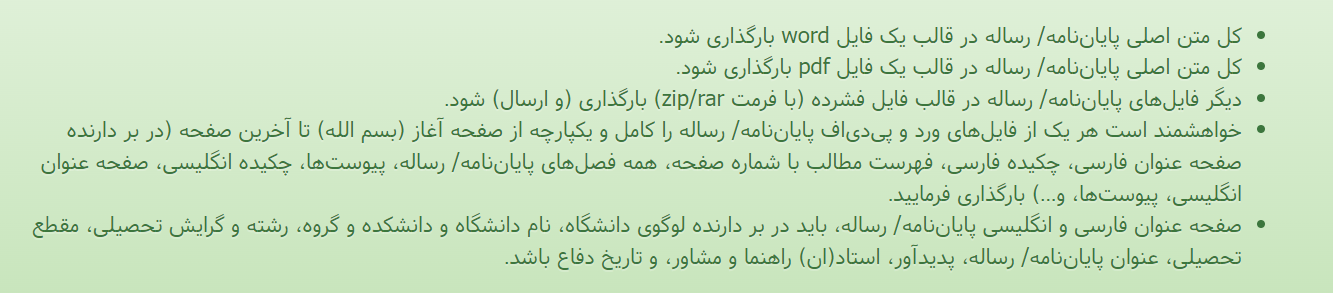
\includegraphics[width = 1\linewidth]{thesis-submission-regulations.png}
	\caption{مقررات مربوط به ثبت پایان‌نامه در ایرانداک} 
	\label{submission-thesis}
\end{figure}


\item \textbf{ثبت در سامانه‌ی 
\href{https://parseh.modares.ac.ir}{پارسه}
:} 
بنابر راهنمای ارسال و بارگذاری پایان‌نامه/رساله در سامانه‌ی پارسه جهت بارگذاری فایل‌های تهیه شده با 
\lr{\LaTeX}،
علاوه بر فایل کامل پایان‌نامه/رساله  با فرمت 
\lr{.pfd}،
یک فایل زیپ شده مربوط به 
\lr{\LaTeX}،
باید یک فایل 
\lr{word} 
 چهار صفحه‌ای به فرمت 
\lr{.doc} 
یا 
\lr{.doxc}
شامل صفحه عنوان فارسی، چکیده‌ی فارسی با کلید واژه‌ها، چکیده‌ی انگلیسی با کلید واژها، صفحه عنوان انگلیسی نیز تهیه و بارگذاری شود. برای اطلاعات بیشتر به 
\linebreak
\href{https://parseh.modares.ac.ir/files/site1/files/guide2.pdf}{راهنمای بارگذاری پایان نامه/ رساله}
مراجعه کنید. 


\item \textbf{مقررات ساختاری در ثبت پایان‌نامه}:
توجه داشته باشید که برای تایید ثبت پایان‌نامه در ایرانداک و همچنین سامانه‌ی پارسه باید حتما پس از صفحه‌ی عنوان، سه فرم را در فایل موجود درج بفرمایید. 
\begin{itemize}
	\item \textbf{برگه‌ی تاییدیه‌ی داوران از جلسه‌ی دفاع:}
توجه داشته باشید این برگه باید توسط استاد راهنما، استاد/اساتید مشاور (در صورت وجود)، نماینده‌ی شورای تحصیلات تکمیلی، داوران داخلی و خارجی به امضا رسیده باشد. 

\item \textbf{آیین‌نامه‌ی حق مالیکت مادی و معنوی:}
		این فرم نیز باید توسط دانشجو تکمیل و امضا شده باشد. 

\item \textbf{آیین‌نامه‌ی حق چاپ :}
		این فرم نیز باید توسط دانشجو تکمیل و امضا شده باشد. 
\end{itemize}
\end{enumerate}	

\noindent
برای دریافت فرم‌های مربوطه به آیین‌نامه‌های ذکر شده در دو مورد آخر به 
\href{https://www.modares.ac.ir/ece/forms}{آدرس فرم‌ها} 
و بخش فرم‌های پژوهشی در دانشکده‌ی مهندسی برق و کامپیوتر دانشگاه تربیت مدرس مراجعه بفرمایید. 

%--------------------------------%
% پیوست‌ها 
\clearpage 
\lhead{ }
\appendix
	
\chapter{ ایجاد پیوست} \label{create appendix}
	
	برای ایجاد پیوست وارد فولدر 
\lr{chapters} 
	بشوید و فایل 
\lr{appendices.tex}
	را باز کنید. توجه داشته باشید که برای ایجاد پیوست حتما در ابتدای فایل دستورات زیر را بکار ببرید (البته اینجا از قبل نوشته شده است). 
	
\begin{latin}
	\begin{verbatim}
		\begin{appendices}
			\chapter{<chapter name 1>}
			\chapter{<chapter name 2>}
		\end{appendices}
	\end{verbatim}
\end{latin} 
	
\chapter{شخصی‌سازی پیوست} \label{option appendix}
	
	برای ایجاد سر‌فصل به نام دلخواه برای پیوست‌ها در فهرست مطالب باید از بسته‌ی 
	\begin{latin}
		\begin{verbatim}
			\package[toc]{appendix}
		\end{verbatim}
	\end{latin} 
	استفاده کنید و اسم مورد نظر برای سرفصل پیوست‌ را با دستور زیر در فایل
	\lr{commands} 
	اعمال کنید. 
	
	\begin{latin}
		\begin{verbatim}
			\renewcommand{\appendixtocname}{<name>}
		\end{verbatim}
	\end{latin} 
	
	برای اطلاعات بیشتر حتما به توضیحات 
	\href{https://ctan.org/pkg/appendix?lang=en}
	{بسته‌ی پیوست} 
	مراجعه بفرمایید. 


%--------------------------------%
% تغییر استایل هدر‌ها به حالت بدون هدر 
\pagestyle{plain}
% تغییر فاصله‌ی بین خطوط 
\linespread{1}
% انتخاب استایل فهرست مراجع 
\bibliographystyle{ieeetr-fa} 
% سایز فونت نرمال 
\normalsize
% چاپ فهرست مراجع 
\printbib
\clearpage
%--------------------------------%
% تغییر فاصله‌ی بین خطوط 
\linespread{1.5}
% کوچکتر کردن سایز فونت 
\small
% چاپ واژه‌نامه 
\printglossary
% چاپ فهرست اختصارات 
\printacronyms
\clearpage
% سایز فونت نرمال 
\normalsize
%--------------------------------%
% تغییر حالت هدر و فوتر به حالت بدون هدر و بدون شماره 
\thispagestyle{empty}
% تک ستونه کردن متن 
\onecolumn
% چکیده‌ی انگلیسی 
%\addcontentsline{toc}{chapter}{\lr{Abstract}}
\begin{latin} 
	\begin{center} 
		\Large{\textbf{Abstract}} \\ \end{center} 
	\linespread{1.4}
	\small	
The abstract goes here. 
	\newline 
	\textbf{\textit{keywords}: First keyword, Second keyword, Third keyword, Forth keyword, Fifth keyword} 
	\normalsize	
\end{latin} 
%--------------------------------%
% صفحه‌ عنوان انگلیسی 
\begin{titlepage}
	\begin{center}
		\begin{figure}[t!]
			\centering
			
\includegraphics[width=0.2\linewidth]{{../images/en_logo.png}}
		\end{figure}
	\begin{latin}
    	{\textbf{Thesis Title}}\\
		\vfill
        Thesis Submitted in Partial Fulfillment of the\\
        Requirements for the Degree of Master of Science (M.Sc.)\\
        in Electrical Engineering, Control System Theory\\
        \vfill
        School of Electrical and Computer Engineering\\
        Tarbiat Modares University\\
		\vfill
		By:\\
		\textbf{Student Name}\\
		\vfill
		Supervisor:\\
		\textbf{Professor name}\\
		\vfill
		\textbf{Season~Year}
		\end{latin}
	\end{center}
\end{titlepage}
%--------------------------------%
%--------------------------------%
\end{document}

